\chapter{Bones}

\keywords{physical pain during meditation}

\noindent Even if we are sitting in good posture, sooner or later,
something somewhere is going to hurt. Practising in a good posture
minimizes unnecessary discomfort, but it can't eliminate it entirely.
Pain and discomfort comes with the fact of having a body, but we are not
meditating to torture ourselves, and we can take care to avoid injury.

Regarding pain in the body, we can either investigate it as a meditation
object, pay attention to another area of the body where there is no
pain, or change our posture.

If our habitual reaction to pain is a sense of anxiety, aversion and
restlessness, then a period of investigation can be useful. Remember the
intention that you wishing yourself well. Then investigate, observe the
pain, how it shifts around in the body, how it arises and ceases in
waves. `Who is suffering? Is it changing? Where is the awareness which
knows this?' This changes our perception from experiencing pain as an
emergency situation which needs to be solved right now, to experiencing
it as a signal which we can choose to put aside for a time.

\enlargethispage*{\baselineskip}

The pain may not be a sign of injury, like, for instance, the discomfort
comparable to what we feel sitting through a long bus ride. We might
choose to keep our attention on a different part of the body. Or we can
move our attention methodically around the body, noticing a spot where
it is not painful, and meditating while staying with the sensations in
that area.

An interesting exercise is to locate exactly where the edges of the
painful area are. Is it a sharp or diffuse boundary? Does it stays
fixed, or does it gradually shift around? This investigation
familiarizes us with the arising and ceasing nature of the pain. It
becomes less of a big deal. We don't have to react with aversion to it,
there can be some free space for the unpleasant sensations to just be.

When you do decide to move, before you move, pause for a moment and
establish a clear intention: `I move out of compassion for the body. I
change posture because I wish my body to be well and healthy.' Then
shift your legs or change posture. This keeps the continuity of
mindfulness intact as we are not then reacting out of aversion or
restlessness.

\keywords{contemplating the body, bones, perception of self}

\enlargethispage*{2\baselineskip}

After a sitting session, you might change the posture to standing, and
allow the joints and the muscles of the body to relax. Standing requires
more attention to maintain balance, and the bones -- the supporting
structures of the body -- are easier to feel.

The bones make up the core, the rigid parts of the body which determine
its shape and what it can and cannot do. Without bones, our body would
be a blob of meat. With bones, it has an inner structure which gives it
the outward appearance we are familiar with. We look in the mirror and
think, `that's me'. How thoroughly did we examine the image before
seeing ourselves in it? A brief glimpse of its outline, contour and
colour will already trigger the perception of `me'. We have a fairly
static image of ourselves, in the present we remember ourselves as an
image from several years ago. Since the rate of change is slow, we rely
on fewer and fewer key features to recognize the image in the mirror.

\clearpage
\thispagestyle{empty}\mbox{}
\contentFullBleed{%
\centering
\null\vfill

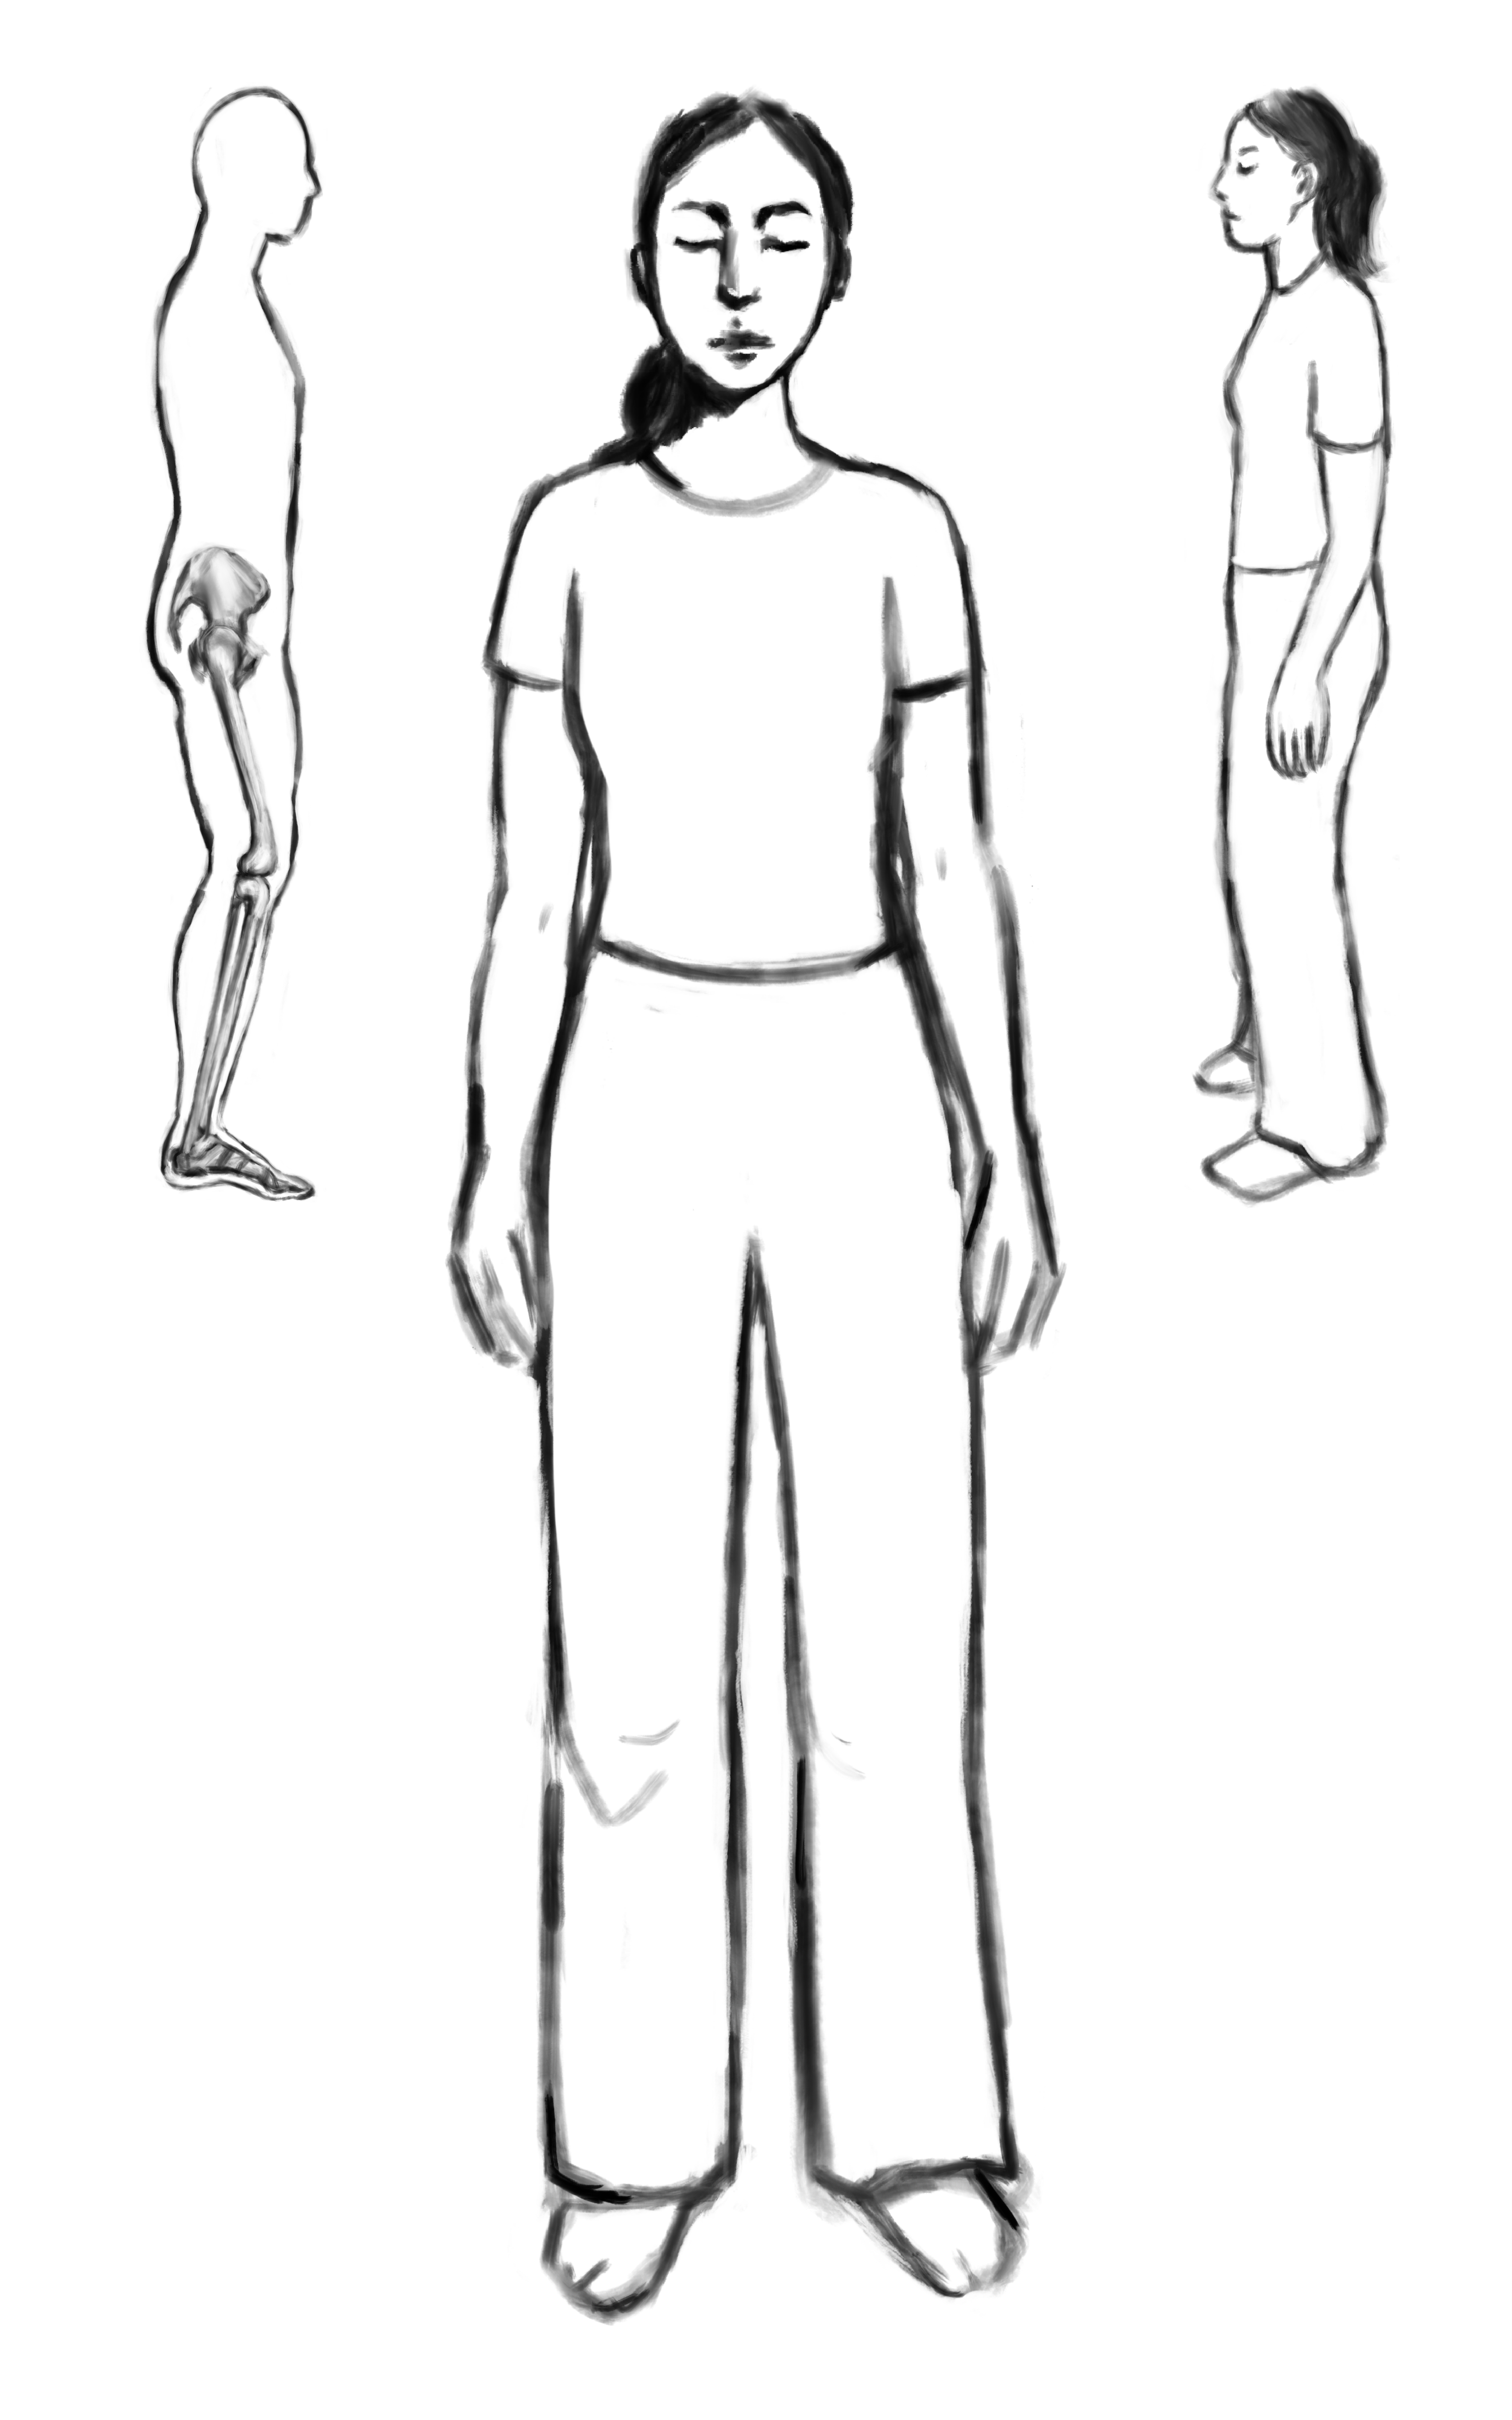
\includegraphics[width=\linewidth-10mm]{standing.png}

\illustration{Standing Meditation Posture}%
\label{illus-standing-meditation}%

\vfill\null
}
\clearpage

Leaning closer, noticing more features, or seeing ourselves from an
unusual angle, it might take minutes to decide who we are looking at.
What determines this image? If the bones were slightly different, the
body would be a different shape. Such a change would change not only our
appearance, but also how we live.

\keywords{standing meditation, standing posture}

Stand in an upright but flexible manner and take some time to find your
balance. Place the feet at shoulder width, with the knees relaxed and
slightly bent, being engaged in holding the body. Don't let the knee
joints lock up straight. This stresses them and will cause your posture
to become rigid. Keep the feet parallel, with the toes pointing straight
ahead. Rotate the hip toward the front along the horizontal axis,
slightly pulling in the lower half. It is a motion like turning a bucket
with the open top turning toward oneself.

Sway the body left and right a bit and feel the centre of weight.
Develop a sense that you are holding the body upright, that you are
preventing it from falling. It is better to balance the weight of the
body toward the heels, rather than leaning on the balls of the feet.

Hold the shoulders wide enough to open the chest for easy breathing, but
not so wide that they become tense. A comfortable place for the hands
can be for example on the thighs, at about over the place where the
pockets are on a pair of jeans.

Allow yourself some flexibility and make small adjustments to your
posture as your muscles get used to the situation. Feel out your balance
in standing and watch, take notice of the body as you hold it this way.
Gravity is pulling it down. There is pressure on the ground. If that's
better, let your hands rest in front of the abdomen, one palm
comfortably on the other.

The eyes may be open or closed. If you feel drowsy, you might prefer
meditating with eyes open, but keep your gaze lowered, looking only a
couple of meters in front of you. If you look straight ahead, your
attention will be directed outwards, and various movements such as those
seen out a window will be distracting.

If you close your eyes but it feels strained and painful, pay attention
to where the eyes are focused when you close them. If they narrow in
close, as if focusing on something close behind the eyelids, this causes
the inner muscles of the eyes to strain and dry. This tension and
dryness can even cause the eyes to water up with tears.

On traditional Buddha statues, the eyes are depicted as being slightly
open. He is awake, not sleeping. Instead of shutting your eyelids tight,
practise relaxing them. Let them stay lowered without any pressure.
Though your eyelids are mostly shut, imagine looking at something far in
distance. This lets the eye muscles relax. To allow some light in, you
can try allowing a narrow slit to remain open. It can also help to
massage the inner eye muscles a bit with the tips of the thumbs in a
circular motion.

Breathe in, and watch how your posture changes with the movement of the
breath. The diaphragm muscle pulls in the air and the abdomen moves
forward to give way. The shoulder bones rise, the ribs in the chest open
outwards, and your body's centre of gravity shifts slightly.

\enlargethispage*{\baselineskip}

Is there something limiting the breathing? Take care to stand upright
and don't let the shoulders hunch as this blocks the open breathing.

Take note of the balance of the head and find the position where the
head sits on top of the spine of its own weight, not leaning forward or
pulled backward. Instead of looking directly ahead, direct your gaze
slightly down in front of you, so as to mitigate your attention becoming
distracted by any comings and goings. Pulling in the chin, direct your
gaze a couple of meters in front of you on the floor. Allow the crown of
your head to rise up a bit, as if pushing the sky.

The position of the head controls the posture of the upper body to a
great degree. Through years of sitting on chairs, we have developed the
habit of pushing our heads forward which creates tension in the back
muscles along the spine. Although we can't control these muscles
consciously, we can experiment. What does it feel like to pull the head
back a bit? You can feel out the balance where the muscles in the back
relax.

In a balanced posture, the vertebrae of the spine sit one on top of
another, like carefully positioned stones. With the spine aligned
upright, gravity is enough to keep it settled in place. Such a posture
gives us a pleasant feeling of light balance without forcing.

\keywords{attitude to the body, analytical mind, goodwill}

If our attitude is too analytical, it can conjure up grotesque and
shocking impressions of the body, but a sense of goodwill towards
ourselves can keep the meditation balanced and wholesome.

The intellect functions by building abstractions and separating out what
it observes. When viewing the body, it might see the various parts as
abstract and inanimate objects. Keep in mind that we are not practising
body-contemplation to create aversion or alienation to the body. We are
practising meditation with clear comprehension in order to see things in
their context, nothing is isolated in a vacuum. Our body-awareness
includes rather than excludes and must come from a welcoming attitude of
acceptance and goodwill.

This difference of attitude reminds me of a story about a dialogue
between Plato and Diogenes. Plato was giving a lecture to his students
at the Academy in Athens, where he defined men as `featherless bipeds'.
Diogenes happened to overhear this and, being fond of practical jokes,
he brought a plucked chicken to Plato and held it up in front of him
proclaiming, `Behold! I've brought you a man.' He must have thought that
this would show that a certain context was lacking in Plato's overly
intellectual definition.

The group at the Academy added `\ldots{} with broad flat nails' to the
definition, in an attempt to satisfy their scholastic sensibilities, but
probably still missing Diogenes' point.

\keywords{experiencing the whole body}

We watch the sensations in the body as we breath in and as we breath
out. Turn attention inwards, mindful of the perception `the body is like
this'. The mind is not seeking, not going off around the world
somewhere. It does not need anything, what is here is enough. Awareness
sees the body, from the feet, to the legs, abdomen, chest, arms,
shoulders, the neck and the head. The body is one whole, one changing
perception, sensitive to the breathing.

\enlargethispage*{\baselineskip}

Watching the body like this is like watching the rain. There is nothing
to do, nothing to decide. The rain just goes on without us having to get
involved.

\clearpage

\keywords{clear comprehension, awareness of the body, defusing anger and desire}

Unskilful thoughts are comparable to dust blowing in the wind: it blocks
our vision, we can't see anything from them. The Buddha compared the
effect of awareness on the mind to rain, as it settles the dust and
clears the air. `Quelling such {[}unskilful{]} thoughts and
considerations, like rain on the dust, with a heart calmed of thought,
you'll touch the state of peace right here.'\footnote{\href{https://suttacentral.net/iti87/en/sujato}{Iti
  87}, Destroyers of Sight}

Awareness of the mind stops unwholesome mind states from arising,
develops wholesome mind states, this way purifying the heart. We may
notice that our experience of the world is not fixed: we are not
isolated outside observers, looking onto a world which is separate from
us. We have a part in creating the world we experience, since we form
its impressions through our mode of attention.

When clear comprehension is established and you notice the mind becoming
more clear and stable, review what allowed this change? What did you do?
What did you \emph{not} do? You didn't have to fight or manipulate the
sense experience or the thoughts and emotions, since they change through
the change in the mode of attention.

Our mode of attention creates the frame of reference from which we
experience the world of the senses, dependent on perception and memory.
This is a process that conditions a certain attitude, like a function
operating over time, which produces how we recognize and interpret
ourselves in the present.

\clearpage

Shifting our mode of attention can serve to stop providing unwholesome
mind states with more fuel. From the perspective of direct experience,
and in accord with the way things are, such unwholesome states are then
denied a basis or reference for their continuance.

In brief, we can say that awareness of the mind purifies the mind.

Staying with the awareness of body defuses both anger and desire. It
changes the frame of our attention and such mind states then fall flat
as though the carpet had been pulled out from under them. The busy,
thinking mind is like a noisy show, or the news in last year's paper.
The topic is no longer interesting, it has lost its urgency, it keeps
going around the same circles. Put the thinking down, like a weary hiker
their heavy backpack, and continue mindful awareness of the body.

Periodic distractions and daydreams can occur, but keep returning to the
breath and the physical sensations of standing. If while standing, you
begin story-telling or fantasizing until the bell rings, that's not
practising insight meditation\ldots{} it is practising waiting for the
bus.

\keywords{memory as self, narratives of self}

\enlargethispage{\baselineskip}

Investigate your state of mind as an experience. The perception of your
body and its feelings arise before we construct the perception of self
from it. What do we remember about ourselves? If we forget about the
narrative that someone told us yesterday, or if we recollect being with
friends years ago, do we perceive ourselves differently?

This interaction between our memories, feelings and mind states keeps
changing. Current perceptions keep changing, and recognizing awareness
places trust in a place which knows this change. This allows us to see
from a wider frame, where there is no fear of the change. Creating the
perception of our self is an ongoing process. We take an active part in
it through actively recalling and re-creating memories. We narrate a
story of ourselves from the memories of the past, and choose choose what
to do now.

\keywords{bones, parts of the body, sense of inadequacy, judgements of appearance}

Observing the body and its parts, our minds stay with the changing
perceptions before the creation of a self. This process disarms the
self-judgement, fears and expectations that bog us down.

Notice the feeling of how the bones connect. There is this perception of
an inner structure which supports the body from the inside: rigid
pieces, connecting end to end, and stacked on top of each other. There
are sensations in the legs: rigid perceptions denoting the long leg
bones. There is pressure. The hip bone is resting on top of the legs and
the torso moves joined above all this. The rib-cage expands and
contracts with the breathing. The spine is holding the weight in a
curve. The head is sitting on top of the spine. The skull bones are
stretching the skin of the face.

\enlargethispage*{\baselineskip}

Our body is made up of pieces. In some places, these pieces are hard and
rigid. In others, they are soft and flexible. The combination of these
is what gives our body its shape. When we look at a person, all we see
is hair of the head, hear of the body, nails, teeth and skin. And we
then construct a person from it all. We glance at a mirror for a
fraction of a second, recognize the general outline or notice some
particular feature, and think, `That's me. How do I look?'

\clearpage

\enlargethispage*{3\baselineskip}

\begin{figure}[h]
\caption{Experience and Illusion of Self}\label{fig-illusion-of-self}

\centering

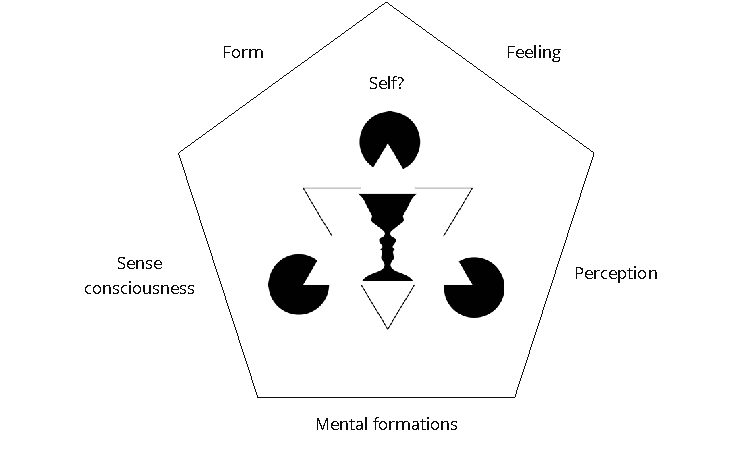
\includegraphics[width=80mm]{./manuscript/tex/diagrams/khandhas-self-illusion.pdf}

\bigskip

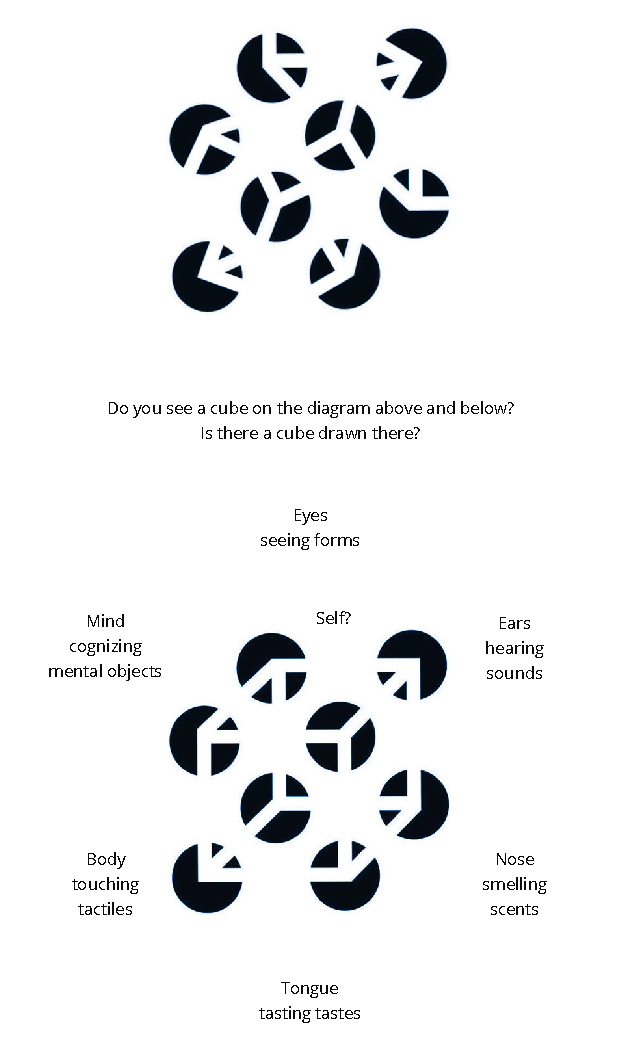
\includegraphics[width=80mm]{./manuscript/tex/diagrams/senses-self-illusion.pdf}

\bigskip

{\small
We experience a self, which has no substance beyond that experience.
Above, conditioned expectations create filled-in shapes which we \emph{experience}, but are not there.
The Kanizsa Triangle, Rubin's Vase and Subjective Necker Cube are examples of illusory contours.
}

\end{figure}

\clearpage

In some situations, we can notice the gradual steps of how this
perception builds up as when we see someone walking in the fog. First,
we recognize the shape of a `person'. Then we detect `male' or `female'.
Maybe it is someone we know? Some detail triggers the final recognition
of our friend and their name. This entire process plays out in the realm
of perception.

The habitual perception of the body -- both of our own body and of other
people's bodies -- is that we see it as one unit, one thing. From that
perspective develops an obsession that there is some ideal way that it
should be. We imagine that the body has to be a certain shape, a certain
size, and so on.

These are worldly judgements, perceptions which our society has drilled
into us. Some cultures idealize a thin body, others a plump one, and
these cultural ideals keep changing from one generation to the next.
Advertisements and various messages from the media reinforce these
expectations and we dutifully believe in them. When we look closer, we
see that such perceptions are twisted and not in accord with reality.

We can be very concerned about what other people think about us, but how
much are \emph{we} concerned about the appearance of others? If I watch
myself, I don't think much about how other people look. But I can feel
self-conscious and imagine that \emph{they} must be thinking about
\emph{me}. When, in fact, they think about me as much as I do of them --
not much, if at all. They are occupied with getting on with their own
life, just as I am with mine.

Besides the pressure of our self-judgment, we imagine how others are
judging us. And since we can't know and can't control what they think,
we internally ruminate in the mind about it, which creates an illusion
of such knowledge and control. When we play out these inner dialogues,
we enjoy the illusion of control. But we miss out on the freedom of
letting go of \emph{the need} for that control.

\keywords{body parts as not-self}

We can notice the conditioned nature of this anxiety when various parts
of the body become detached. We can be so concerned about our hair, for
example\ldots{} but only when it is on our head. When the hairdresser
cuts it off, we are not anxious about the pile of hair on the floor.
Similarly, when cutting our nails, what is that point when it is no
longer `me' and `mine'?

When we contemplate the body in this way, we see it not as one unit, but
as made up of pieces and parts which have their own nature and behave
accordingly, each part not the least concerned with our opinions or
those of others. Bones, skin, hair, teeth and nails: they are the way
they are.

The body is a blessing. This meditation is not meant to develop aversion
toward the body. Health is a blessing, it supports us in everything we
do. The Buddha called health the greatest treasure.

\keywords{stories as dreams, awareness of the body, grey and drifting states, gratitude}

We observe the breath, the parts of the body, and our present
experience. When we look, we find that they don't carry the stories of
`me' and `mine' with them. Since it is we who are creating these
stories, we can also stop creating them, we are not chained to following
them. Phenomena arise through dependent conditions. When the conditions
cease, the phenomena cease. This is all that happens.

Awareness of the body loosens the grip of our desires and leads us to
recognize that we are fortunate to be here. We can always return to this
attention: one in-breath and out-breath is enough to remember arising
and ceasing. Doubts become like stories in an old newspaper. We get
tired of untangling the threads of the past which are so difficult to
follow. It is like interpreting someone else's dreams.

What is real, is always here in our present experience. What becomes
important is not who or what we are in the story, but whether we can
give our attention to where we are now.

Clear intention has an important role. When we don't set a clear
intention, we are drifting. Perhaps we don't particularly mind being
here and drifting like this, but the mind is grey with no life, almost
trying to hide itself and be invisible. We end up being grey and
invisible like that. Nothing wrong is happening, but there isn't any
brightness and joy in being here.

We don't stop often enough to notice when we are happy and peaceful.
When the mind is clear and calm, the natural feeling is a sense of
gratitude for what is here, and for the blessings we have received in
our life.

\enlargethispage*{\baselineskip}

Gratitude is not created by will. In this practice we are not creating
anything, we simply recognize what is here with clear intention. It is
not a matter of strength or ability as those are bound to time and
circumstance. But resolution and mindful attention are not bound to a
given circumstance. The result is a right perspective in which we can
see the right order of things and what to do with them -- or to stop,
give attention and breathe.
